\documentclass{cshwk}

\begin{document}
\title{HW \#1, Chapter 1}
\maketitle


\section{Problem 3. Chapter 1 P18}
Perform a Traceroute between source and destination on the same continent at three different hours of the day.

a. Find the average and standard deviation of the round-trip delays at each of the three hours.

b. Find the number of routers in the path at each of the three hours. Did the paths change during any of the hours?

c. Try to identify the number of ISP networks that the Traceroute packets pass through from source to destination. Routers with similar names and/or similar IP addresses should be considered as part of the same ISP. In your experiments, do the largest delays occur at the peering interfaces between adjacent ISPs?

d. Repeat the above for a source and destination on different continents. Compare the intra-continent and inter-continent results.
\subsection*{Solutions:}

The \texttt{Traceroute} package in \texttt{ArchLinux} can be used to perform network route tracing. Installing this package by running command:
\begin{verbatim}
    yay -S traceroute
\end{verbatim}
After installing, we can use the command:
\begin{verbatim}
    sudo traceroute -A -I -T <destination>
\end{verbatim}
Where the arguments are:
\begin{itemize}
    \item \texttt{-A}: Displays Autonomous System (AS) numbers.
    \item \texttt{-I}: Uses ICMP Echo Request packets. (like command \texttt{ping})
    \item \texttt{-T}: Uses TCP SYN packets, which simulate the start of a TCP connection. This can bypass firewalls or NATs that block UDP or ICMP but allow TCP traffic.
    \item \texttt{<destination>}: The destination address.
\end{itemize}
While located at my home in Beijing, I used the \texttt{traceroute} command to trace two of my VPS servers on different continents at three different times during the day (morning, afternoon, and night). Servers are:
\begin{itemize}
    \item \texttt{subit.org.cn (47.95.10.252)}: Aliyun server in Beijing, China.
    \item \texttt{steven12138.xyz (45.76.203.208)}: Vultr server in Japan.
\end{itemize}
After running these analyses at \texttt{10:28}, \texttt{14:09}, and \texttt{16:05} on \texttt{2024-09-22}, the results are shown in Fig..~\ref{fig:traceroute1}-\ref{fig:traceroute6} in the Appendix.

Now, let's analyze the results:

\subsubsection*{A. Average and Standard Deviation of the Round-Trip Delays}
The average and standard deviation of the round-trip delays at each of the three hours are shown in Tab.~\ref{tab:delay}.
\begin{table}[H]
    \centering
    \begin{tabular}{ccc}
        \hline
        Time  & Beijing (ms) & Tokyo (ms) \\
        \hline
        10:28 & $27.925$     & $71.856$   \\
        14:09 & $36.086$     & $71.146$   \\
        16:05 & $30.510$     & $71.048$   \\
        \hline
    \end{tabular}
    \caption{Average and standard deviation of the round-trip delays}
    \label{tab:delay}
\end{table}

\textbf{Therefore, the average and standard deviation of the round-trip delays at each of the three hours are shown in Tab.~\ref{tab:delay_result}.}
\begin{table}[H]
    \centering
    \begin{tabular}{ccc}
        \hline
        Location & Average (ms) & Standard Deviation (ms) \\
        \hline
        Beijing  & $31.5070$    & $3.4055$                \\
        Tokyo    & $71.0167$    & $0.6985$                \\
        \hline
    \end{tabular}
    \caption{Average and standard deviation of the round-trip delays}
    \label{tab:delay_result}
\end{table}

\subsubsection*{B. Number of Routers in the Path}
The number of routers in the path at each of the three hours are shown in Tab.~\ref{tab:routers}.
\begin{table}[H]
    \centering
    \begin{tabular}{ccc}
        \hline
        Time  & Beijing & Tokyo \\
        \hline
        10:28 & $11$    & $14$  \\
        14:09 & $11$    & $14$  \\
        16:05 & $11$    & $14$  \\
        \hline
    \end{tabular}
    \caption{Number of routers in the path}
    \label{tab:routers}
\end{table}
We can also draw the route path of the traceroute (identified nodes only) in Fig.~\ref{fig:route}.
\begin{figure}[htbp]
    \centering
    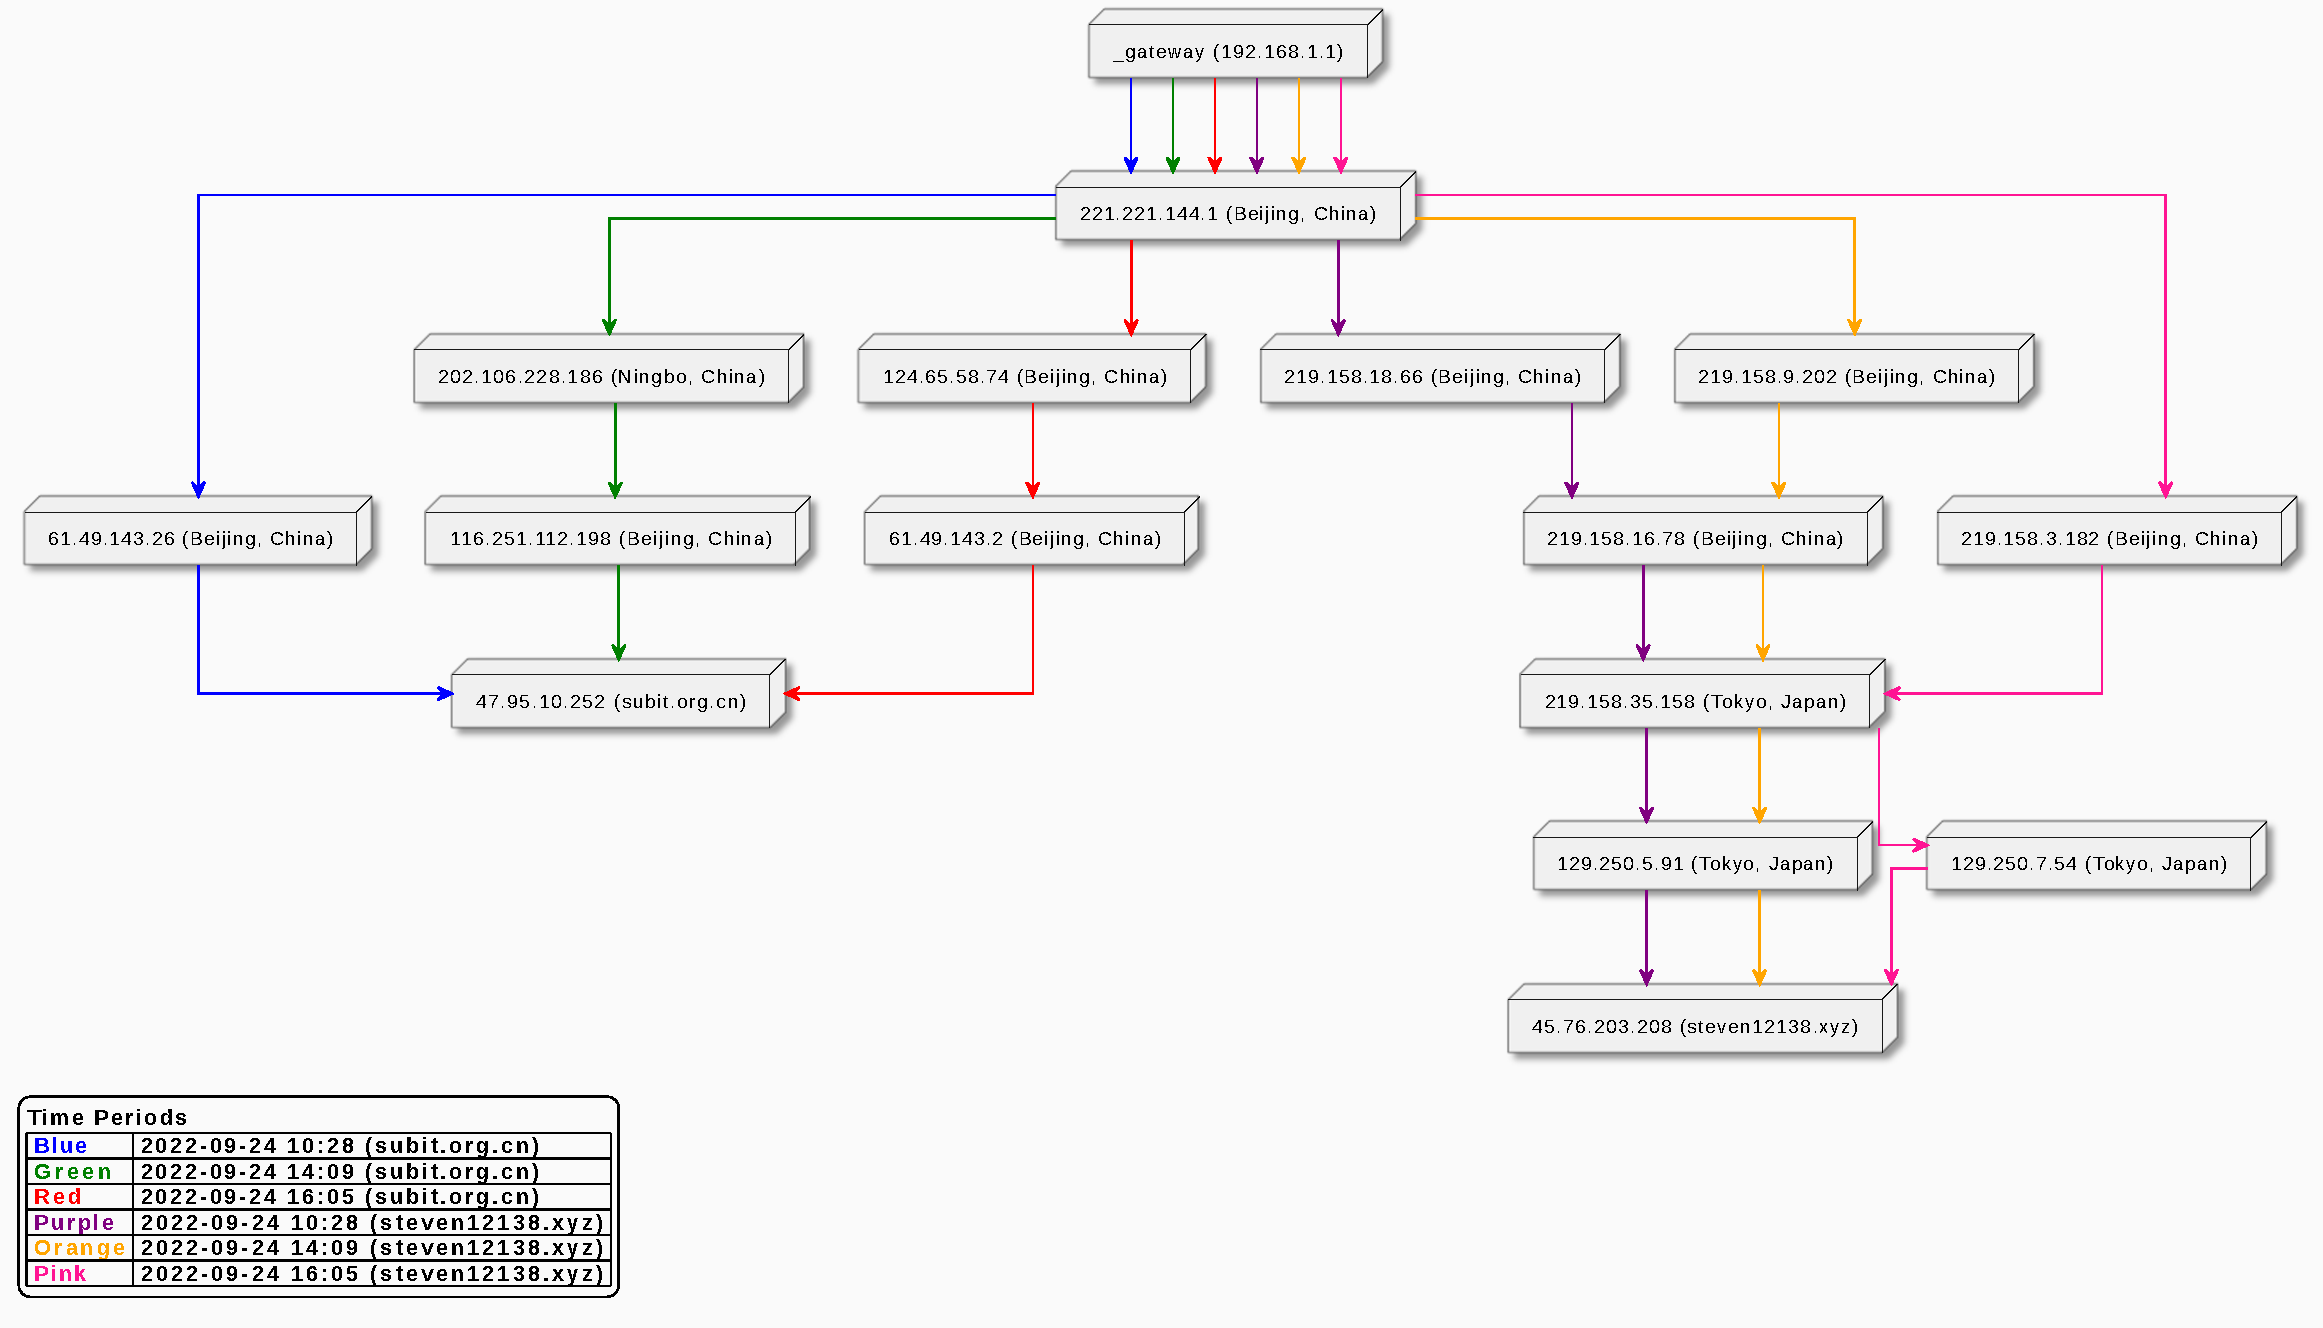
\includegraphics[width=1\textwidth]{./hw1-3-1.pdf}
    \caption{Route path of the traceroute}
    \label{fig:route}
\end{figure}
\textbf{We can see that the paths do change during any of the hours.}

\subsubsection*{C. Identify the Number of ISP Networks}
We use the \texttt{-A} option in the \texttt{traceroute} command to display Autonomous System (AS) numbers. And we can find the ISP of the AS numbers by running command:
\begin{verbatim}
    whois -h whois.cymru.com " -v AS<AS Number>"
\end{verbatim}
The routes to the Aliyun Beijing server using the the AS number \texttt{AS4808}, \texttt{AS37963}. The whois results are shown in Tab.~\ref{tab:AS_result_aliyun}.
\begin{table}[H]
    \centering
    \begin{tabular}{cccp{3in}}
        \hline
        AS Number & CC & Registry & Name                                                     \\
        \hline
        4808      & CN & apnic    & CHINA169-BJ China Unicom Beijing Province Network, CN    \\
        37963     & CN & apnic    & ALIBABA-CN-NET Hangzhou Alibaba Advertising Co.,Ltd., CN \\
        \hline
    \end{tabular}
    \caption{The ISP Info of the routes to the Aliyun Beijing server}
    \label{tab:AS_result_aliyun}
\end{table}

The routes to the Vultr Japan server using the the AS number \texttt{AS4808}, \texttt{AS4837}, \texttt{AS2914}, \texttt{AS20473}. The whois results are shown in Tab.~\ref{tab:AS_result_vultr}.
\begin{table}[H]
    \centering
    \begin{tabular}{cccp{3in}}
        \hline
        AS Number & CC & Registry & Name                                                  \\
        \hline
        4808      & CN & apnic    & CHINA169-BJ China Unicom Beijing Province Network, CN \\
        4837      & CN & apnic    & CHINA169-BACKBONE CHINA UNICOM China169 Backbone, CN  \\
        2914      & US & arin     & NTT-LTD-2914, US                                      \\
        20473     & US & arin     & AS-VULTR, US                                          \\
        \hline
    \end{tabular}
    \caption{The ISP Info of the routes to the Vultr Japan server}
    \label{tab:AS_result_vultr}
\end{table}

By analyzing the results, we observe that the largest delays occur at peering interfaces between adjacent ISPs when routing to the Aliyun server. However, these delays are not the most significant when routing to the Vultr server.

For the Vultr server, the maximum delay occurs between the 6th and 7th hops, both belonging to the same ISP. An IP lookup reveals that the 6th hop is located in Beijing, while the 7th hop is in Tokyo. This delay could be attributed to the long distance between Beijing and Tokyo, despite the existence of undersea optical cables connecting them.

The Great Firewall (GFW) of China may also contribute to the delay. It is a combination of legislative measures and technologies enforced by the People's Republic of China to regulate domestic Internet access. Its role in Internet censorship includes blocking access to selected foreign websites and slowing down cross-border internet traffic.

The GFW employs Deep Packet Inspection (DPI) technology to detect and block certain types of traffic. DPI inspects the data portion (and sometimes the header) of packets as they pass through a checkpoint, searching for protocol violations, viruses, spam, intrusions, or other predefined criteria. Based on this inspection, packets may be allowed through, rerouted, or blocked entirely. This process can contribute to traffic delays.

In conclusion, the delay is a multifactorial issue, likely caused by the long distance between the source and destination, peering interfaces between adjacent ISPs, and local government policies like the GFW.


\subsubsection*{D. Intra-continent and Inter-continent Results}

Furthermore, we trace the routes to official website of the University of Tokyo, the University of Illinois, ETH Zurich, and the University of Cambridge, which are located on different continents.The results are shown in Fig.~\ref{fig:traceroute-utokyo}-\ref{fig:traceroute-cambridge} in the Appendix.

The summary of the results are shown in Tab.~\ref{tab:summary}.
\begin{table}[H]
    \centering
    \begin{tabular}{cccc}
        \hline
        Country & University              & Delay (ms) & Number of the routes \\
        \hline  
        JP      & University of Tokyo     & $381.651$  & $18$                 \\
        USA     & University of Illinois  & $226.336$  & $26$                 \\
        EU      & ETH Zurich              & $306.731$  & $21$                 \\
        UK      & University of Cambridge & $259.840$  & $26$                 \\
        \hline
    \end{tabular}
    \caption{Summary of the results}
    \label{tab:summary}
\end{table}

The routing path is shown in Fig.~\ref{fig:route-diff-continent}. Different color represents different route trace. We can anaylsis from the figure that the path to EU, UK and US are similar. They all go through the United States, but the path to University of Illinois stops in the US while others keep go through the Europe or UK. That's why the delay to University of Illinois is significantly lower than the others. Moreover, the path to the University of Tokyo is the longest, which brings the largest delay. 

\begin{figure}[H]
    \centering
    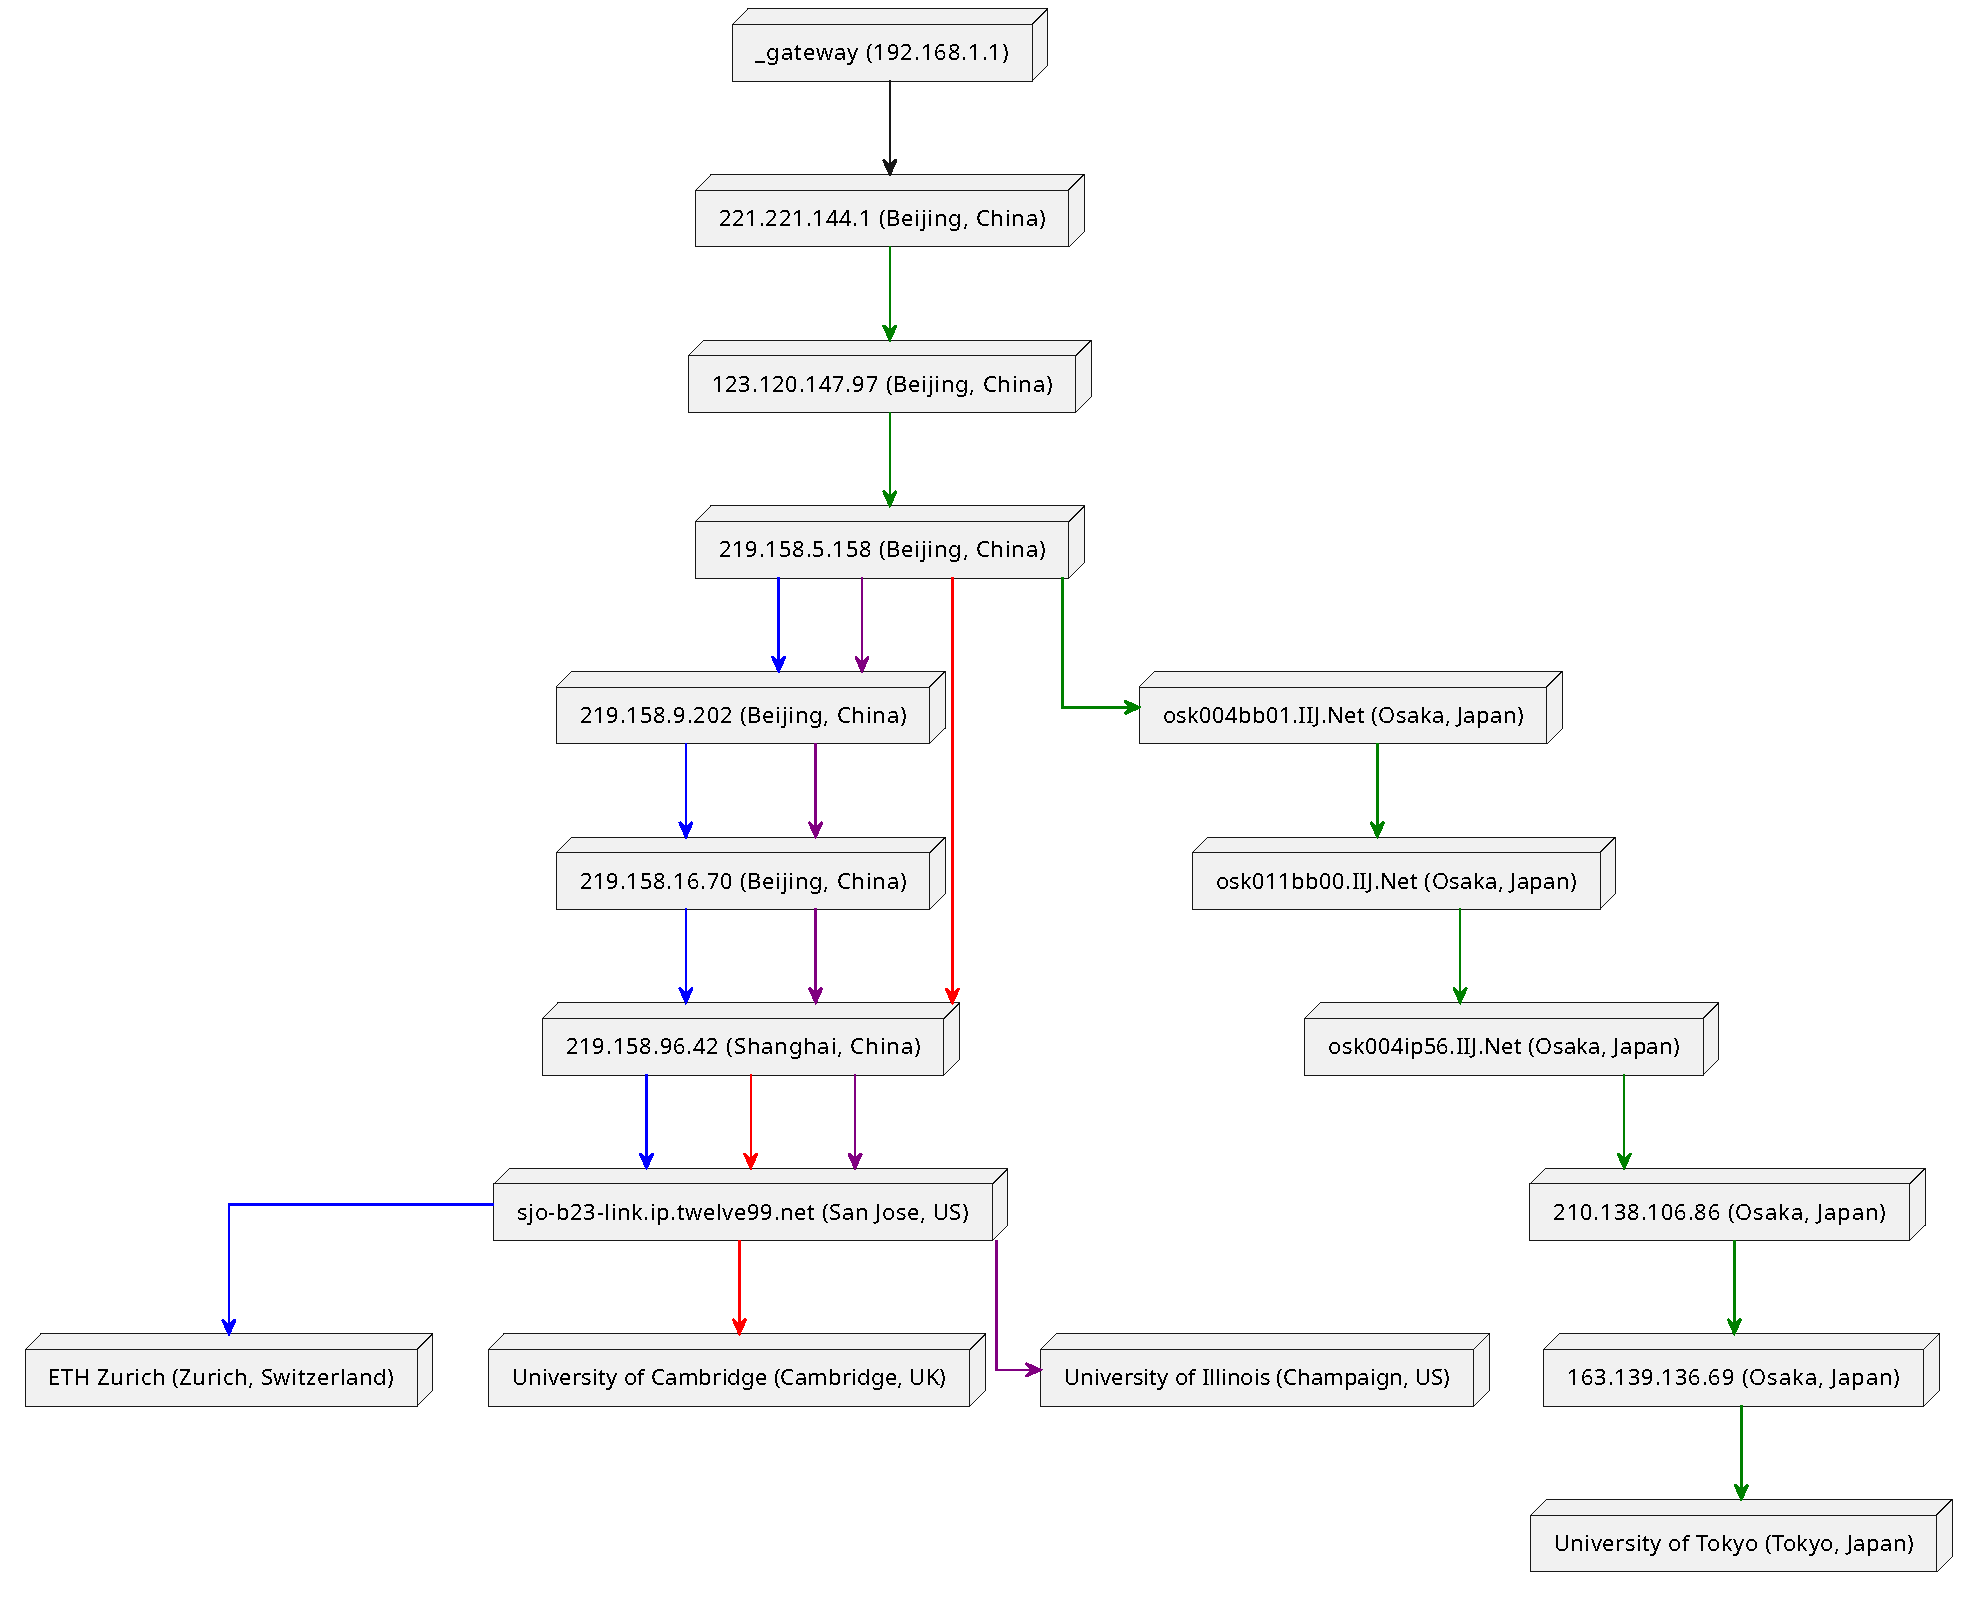
\includegraphics[width=0.8\textwidth]{hw1-3-2.pdf}
    \caption{Route path of the traceroute to different continents}
    \label{fig:route-diff-continent}
\end{figure}

\newpage
\section{Appendix}


\subsection{Three Different Hours of the Day Results}
\begin{figure}[H]
    \footnotesize
    \begin{verbatim}
        traceroute to steven12138.xyz (45.76.203.208), 30 hops max, 60 byte packets
        1  _gateway (192.168.1.1) [*]  2.285 ms  3.126 ms *
        2  221.221.144.1 (221.221.144.1) [AS4808]  9.878 ms * *
        3  * * *
        4  * * *
        5  * * 219.158.18.66 (219.158.18.66) [AS4837]  10.970 ms
        6  219.158.16.78 (219.158.16.78) [AS4837]  11.790 ms * *
        7  219.158.35.158 (219.158.35.158) [AS4837]  78.290 ms * *
        8  ae-25.r33.tokyjp05.jp.bb.gin.ntt.net (129.250.5.200) [AS2914]  72.845 ms * *
        9  * ae-10.a01.tokyjp09.jp.bb.gin.ntt.net (129.250.5.91) [AS2914]  70.963 ms *
       10  ce-3-5-3.a01.tokyjp09.jp.ce.gin.ntt.net (120.88.54.98) [AS2914]  70.916 ms * *
       11  * * *
       12  * * *
       13  * * *
       14  45.76.203.208.vultrusercontent.com (45.76.203.208) [AS20473]  71.856 ms * *             
    \end{verbatim}
    \caption{Vultr Japan server on \texttt{2024-09-22 10:28}}
    \label{fig:traceroute1}
\end{figure}

\begin{figure}[H]
    \footnotesize
    \begin{verbatim}
        traceroute to subit.org.cn (47.95.10.252), 30 hops max, 60 byte packets
        1  _gateway (192.168.1.1) [*]  14.498 ms  14.560 ms *
        2  221.221.144.1 (221.221.144.1) [AS4808]  17.860 ms * *
        3  * * *
        4  * * *
        5  * 61.49.143.26 (61.49.143.26) [AS4808]  21.296 ms *
        6  * * *
        7  * * *
        8  * * *
        9  * * *
        10  * * *
        11  47.95.10.252 (47.95.10.252) [AS37963]  27.925 ms * *
    \end{verbatim}
    \caption{Aliyun Beijing server on \texttt{2024-09-22 10:28}}
\end{figure}

\begin{figure}[H]
    \footnotesize
    \begin{verbatim}
        traceroute to steven12138.xyz (45.76.203.208), 30 hops max, 60 byte packets
        1  _gateway (192.168.1.1) [*]  1.605 ms  1.737 ms *
        2  221.221.144.1 (221.221.144.1) [AS4808]  5.787 ms * *
        3  * * *
        4  * * *
        5  * 219.158.9.202 (219.158.9.202) [AS4837]  7.822 ms *
        6  219.158.16.78 (219.158.16.78) [AS4837]  14.441 ms * *
        7  219.158.35.158 (219.158.35.158) [AS4837]  79.069 ms * *
        8  * * *
        9  * * ae-10.a01.tokyjp09.jp.bb.gin.ntt.net (129.250.5.91) [AS2914]  69.428 ms
        10  ce-3-5-3.a01.tokyjp09.jp.ce.gin.ntt.net (120.88.54.98) [AS2914]  71.094 ms * *
        11  * * *
        12  * * *
        13  * * *
        14  45.76.203.208.vultrusercontent.com (45.76.203.208) [AS20473]  70.146 ms * *
    \end{verbatim}
    \caption{Vultr Japan server on \texttt{2024-09-22 14:09}}
\end{figure}

\begin{figure}[H]
    \footnotesize
    \begin{verbatim}
        traceroute to subit.org.cn (47.95.10.252), 30 hops max, 60 byte packets
        1  _gateway (192.168.1.1) [*]  2.205 ms  2.338 ms *
        2  221.221.144.1 (221.221.144.1) [AS4808]  5.558 ms * *
        3  * * *
        4  * bt-228-186.bta.net.cn (202.106.228.186) [AS4808]  6.786 ms *
        5  * * *
        6  116.251.112.198 (116.251.112.198) [AS45102]  29.336 ms * *
        7  * * *
        8  * * *
        9  * * *
        10  * * *
        11  47.95.10.252 (47.95.10.252) [AS37963]  36.086 ms * *
    \end{verbatim}
    \caption{Aliyun Beijing server on \texttt{2024-09-22 14:09}}
\end{figure}

\begin{figure}[H]
    \footnotesize
    \begin{verbatim}
        traceroute to steven12138.xyz (45.76.203.208), 30 hops max, 60 byte packets
        1  _gateway (192.168.1.1) [*]  8.184 ms  8.260 ms  7.176 ms
        2  221.221.144.1 (221.221.144.1) [AS4808]  10.703 ms * *
        3  * * *
        4  * 125.33.186.137 (125.33.186.137) [AS4808]  11.625 ms *
        5  * * *
        6  219.158.3.182 (219.158.3.182) [AS4837]  13.626 ms * *
        7  219.158.35.158 (219.158.35.158) [AS4837]  68.855 ms * *
        8  * * *
        9  * ae-0.a01.tokyjp09.jp.bb.gin.ntt.net (129.250.7.54) [AS2914]  75.529 ms *
        10  ce-3-5-3.a01.tokyjp09.jp.ce.gin.ntt.net (120.88.54.98) [AS2914]  76.799 ms * *
        11  * * *
        12  * * *
        13  * * *
        14  45.76.203.208.vultrusercontent.com (45.76.203.208) [AS20473]  71.048 ms 
            71.001 ms  71.104 ms
    \end{verbatim}
    \caption{Vultr Japan server on \texttt{2024-09-22 16:05}}
\end{figure}

\begin{figure}[H]
    \footnotesize
    \begin{verbatim}
        traceroute to subit.org.cn (47.95.10.252), 30 hops max, 60 byte packets
        1  _gateway (192.168.1.1) [*]  6.645 ms  9.661 ms *
        2  221.221.144.1 (221.221.144.1) [AS4808]  12.372 ms * *
        3  * * *
        4  * * 124.65.58.74 (124.65.58.74) [AS4808]  13.482 ms
        5  * * 61.49.143.2 (61.49.143.2) [AS4808]  13.962 ms
        6  * * *
        7  * * *
        8  * * *
        9  * * *
        10  * * *
        11  * * 47.95.10.252 (47.95.10.252) [AS37963]  30.510 ms
    \end{verbatim}
    \caption{Aliyun Beijing server on \texttt{2024-09-22 16:05}}
    \label{fig:traceroute6}
\end{figure}

\subsection{Different continents results}

\begin{figure}[H]
    \footnotesize
    \begin{verbatim}
        traceroute to www.u-tokyo.ac.jp (210.152.243.234), 30 hops max, 60 byte packets
        1  _gateway (192.168.1.1) [*]  3.220 ms  3.437 ms *
        2  221.221.144.1 (221.221.144.1) [AS4808]  6.882 ms * *
        3  123.120.147.97 (123.120.147.97) [AS4808]  7.024 ms * *
        4  * * *
        5  * 219.158.5.158 (219.158.5.158) [AS4837]  12.706 ms *
        6  219.158.3.146 (219.158.3.146) [AS4837]  14.152 ms * *
        7  * * *
        8  193.251.145.107 (193.251.145.107) [AS5511]  149.034 ms * *
        9  * * *
        10  * * *
        11  * * *
        12  * osk004bb01.IIJ.Net (58.138.88.117) [AS2497]  229.146 ms 
          osk011bb00.IIJ.Net (58.138.84.169) [AS2497]  253.227 ms
        13  * osk004ip56.IIJ.Net (58.138.81.66) [AS2497]  255.221 ms *
        14  210.138.106.86 (210.138.106.86) [AS2497]  310.369 ms * *
        15  * 163.139.136.69 (163.139.136.69) [AS2519]  311.345 ms *
        16  * * 222.230.187.142 (222.230.187.142) [AS2519]  317.842 ms
        17  * * *
        18  210-152-243-234.jp-west.compute.idcfcloud.com (210.152.243.234) [AS4694]  
          381.651 ms * *
    \end{verbatim}
    \caption{University of Tokyo}
    \label{fig:traceroute-utokyo}
\end{figure}

\begin{figure}[H]
    \footnotesize
    \begin{verbatim}
        traceroute to illinois.edu (130.126.157.20), 30 hops max, 60 byte packets
        1  _gateway (192.168.1.1) [*]  1.877 ms  1.837 ms  0.986 ms
        2  221.221.144.1 (221.221.144.1) [AS4808]  4.245 ms * *
        3  221.223.117.245 (221.223.117.245) [AS4808]  4.434 ms * *
        4  * * *
        5  219.158.5.146 (219.158.5.146) [AS4837]  8.162 ms * *
        6  219.158.9.237 (219.158.9.237) [AS4837]  10.680 ms * *
        7  219.158.16.98 (219.158.16.98) [AS4837]  161.115 ms * *
        8  lax-b3-link.ip.twelve99.net (80.239.134.246) [AS1299]  213.843 ms * *
        9  lax-b22-link.ip.twelve99.net (62.115.126.248) [AS1299]  306.418 ms * *
        10  * * *
        11  * * *
        12  chi-bb1-link.ip.twelve99.net (62.115.113.75) [AS1299]  244.244 ms 
            244.664 ms  244.606 ms
        13  chi-b24-link.ip.twelve99.net (62.115.115.71) [AS1299]  215.731 ms 
            307.357 ms  307.278 ms
        14  wiscnet-ic-369229.ip.twelve99-cust.net (213.248.71.113) [AS1299]  307.207 ms
            306.538 ms  306.493 ms
        15  t-ur1rtr.ix.ui-iccn.org (72.36.127.86) [AS40387/AS198949]  306.273 ms
            306.220 ms  306.195 ms
        16  t-ur1rtr.ix.ui-iccn.org (72.36.127.86) [AS40387/AS198949]  306.171 ms
            72.36.126.233 (72.36.126.233) [AS40387/AS198949]  306.347 ms
            t-ur1rtr.ix.ui-iccn.org (72.36.127.86) [AS40387/AS198949]  306.123 ms
        17  t-rtr-urbexit1.gw.uiuc.edu (130.126.0.201) [AS38/AS198949]  306.301 ms
            306.279 ms t-rtr-urbexit1.gw.uiuc.edu (72.36.127.2) [AS40387/AS198949]  311.207 ms
        18  t-rtr-urbexit1.gw.uiuc.edu (130.126.0.201) [AS38/AS198949]  311.136 ms 
            t-fw-urbexit.gw.uiuc.edu (130.126.0.142) [AS38/AS198949]  311.137 ms  311.104 ms
        19  t-rtr-urbexit1.gw.uiuc.edu (130.126.0.133) [AS38/AS198949]  307.664 ms  307.572 ms 
            t-fw-urbexit.gw.uiuc.edu (130.126.0.142) [AS38/AS198949]  307.539 ms
        20  t-rtr-brdrdist2.gw.uiuc.edu (130.126.1.114) [AS38/AS198949]  307.465 ms 
            t-rtr-urbexit1.gw.uiuc.edu (130.126.0.133) [AS38/AS198949]  307.452 ms  307.417 ms
        21  t-rtr-brdrdist9.gw.uiuc.edu (130.126.1.126) [AS38/AS198949]  307.302 ms * 
            t-rtr-brdrdist2.gw.uiuc.edu (130.126.1.114) [AS38/AS198949]  307.297 ms
        22  * * *
        23  * * *
        24  * * *
        25  alma.techservices.illinois.edu (130.126.157.20) [AS38/AS198949]  226.336 ms * *
    \end{verbatim}
    \caption{University of Illinois}
    \label{fig:traceroute-uiuc}
\end{figure}

\begin{figure}[H]
    \footnotesize
    \begin{verbatim}
        traceroute to ethz.ch (129.132.19.216), 30 hops max, 60 byte packets
        1  _gateway (192.168.1.1) [*]  1.720 ms  1.777 ms *
        2  221.221.144.1 (221.221.144.1) [AS4808]  8.561 ms * *
        3  * * *
        4  * * *
        5  * 219.158.9.202 (219.158.9.202) [AS4837]  11.178 ms *
        6  219.158.16.70 (219.158.16.70) [AS4837]  14.666 ms * *
        7  219.158.96.42 (219.158.96.42) [AS4837]  273.432 ms * *
        8  sjo-b23-link.ip.twelve99.net (80.239.135.4) [AS1299]  204.989 ms * *
        9  * * nyk-bb2-link.ip.twelve99.net (62.115.119.228) [AS1299]  306.781 ms
        10  * * ldn-bb2-link.ip.twelve99.net (62.115.139.247) [AS1299]  306.874 ms
        11  prs-bb2-link.ip.twelve99.net (62.115.133.239) [AS1299]  306.886 ms * *
        12  ffm-bb2-link.ip.twelve99.net (62.115.122.139) [AS1299]  307.005 ms * *
        13  zch-b1-link.ip.twelve99.net (62.115.138.47) [AS1299]  306.364 ms * *
        14  dante-ic-383626.ip.twelve99-cust.net (213.248.79.190) [AS1299]  307.053 ms * *
        15  swiEZ2-B3.switch.ch (130.59.36.176) [AS559]  315.127 ms * *
        16  swiEZ3-B1.switch.ch (130.59.36.126) [AS559]  331.600 ms * *
        17  rou-gw-lee-tengig-to-switch.ethz.ch (192.33.92.1) [AS559]  312.188 ms * *
        18  rou-fw-rz-rz-gw.ethz.ch (192.33.92.169) [AS559]  344.007 ms * *
        19  * * lb-lee-service-id-bd-unix-lb-out-1.ethz.ch (129.132.19.195) [AS559]  306.816 ms
        20  * * *
        21  cms-publish.ethz.ch (129.132.19.216) [AS559]  306.731 ms * *
    \end{verbatim}
    \caption{ETH Zurich}
    \label{fig:traceroute-ethz}
\end{figure}

\begin{figure}[H]
    \footnotesize
    \begin{verbatim}
        traceroute to www.cam.ac.uk (128.232.132.8), 30 hops max, 60 byte packets
        1  _gateway (192.168.1.1) [*]  1.040 ms *  1.176 ms
        2  * * 221.221.144.1 (221.221.144.1) [AS4808]  5.436 ms
        3  * * *
        4  * * *
        5  * * *
        6  219.158.8.122 (219.158.8.122) [AS4837]  44.385 ms * *
        7  219.158.103.26 (219.158.103.26) [AS4837]  43.993 ms * *
        8  219.158.20.178 (219.158.20.178) [AS4837]  203.784 ms * *
        9  219.158.34.242 (219.158.34.242) [AS4837]  203.746 ms * *
        10  ffm-bb1-link.ip.twelve99.net (62.115.124.116) [AS1299]  203.751 ms * *
        11  prs-bb2-link.ip.twelve99.net (62.115.122.138) [AS1299]  203.753 ms * *
        12  ldn-bb2-link.ip.twelve99.net (62.115.133.238) [AS1299]  204.722 ms * *
        13  ldn-b11-link.ip.twelve99.net (62.115.138.169) [AS1299]  203.656 ms * *
        14  * * jisc-ic-345130.ip.twelve99-cust.net (62.115.175.107) [AS1299]  242.488 ms
        15  ae24.londtt-sbr1.ja.net (146.97.35.193) [AS786]  244.578 ms * *
        16  ae28.londtw-sbr2.ja.net (146.97.33.62) [AS786]  248.205 ms * *
        17  ae31.lowdss-sbr1.ja.net (146.97.33.29) [AS786]  283.699 ms * *
        18  ae26.lowdss-ban1.ja.net (146.97.35.246) [AS786]  271.630 ms * *
        19  uoc.ja.net (146.97.41.38) [AS786]  271.927 ms * *
        20  c-hi.b-jc.net.cam.ac.uk (131.111.7.82) [AS786]  247.351 ms * *
        21  * * *
        22  reserved.net.cam.ac.uk (128.232.197.71) [AS786]  306.530 ms * *
        23  reserved.net.cam.ac.uk (128.232.197.65) [AS786]  306.562 ms * *
        24  s-dw.f-sv-net.net.cam.ac.uk (128.232.128.2) [AS786]  306.511 ms * *
        25  f-sv-net.f-sv-uis.net.cam.ac.uk (128.232.128.10) [AS786]  306.431 ms * *
        26  * tm-128-232-132-8.tm.uis.cam.ac.uk (128.232.132.8) [AS786]  259.840 ms *
    \end{verbatim}
    \caption{University of Cambridge}
    \label{fig:traceroute-cambridge}
\end{figure}

\end{document}